\documentclass[12pt,a4paper]{article}
\usepackage{acro,hyperref,graphicx}
\usepackage[margin=1in]{geometry}

\usepackage[british]{babel}
\usepackage[style=apa]{biblatex}
\DeclareLanguageMapping{british}{british-apa}

\addbibresource{./refs.bib}

\hypersetup{
    bookmarks=true,
    unicode=false,
    pdftoolbar=true,
    pdfmenubar=true,
    pdffitwindow=false,
    pdfstartview={FitH},
    pdftitle={Social Network Analysis in English Literature},
    pdfauthor={Sean Allred},
    pdfsubject={Research},
    pdfkeywords={research} {nltk},
    pdfnewwindow=true,
    colorlinks=true,
    linkcolor=black,%red,
    citecolor=black,%magenta,
    filecolor=black,%magenta,
    urlcolor=black%cyan
}

\DeclareAcronym{nltk}{
  short=NLTK,
  long=Natural Language Toolkit,
  short-indefinite=the,
  long-indefinite=the
}

\title{Social Network Analysis\\[-18pt]in English Literature\\{\large
    SCI30010 Assignment 1}} \author{Sean Allred} \date{\today}

\renewcommand{\abstractname}{Problem Statement and Goal}

\linespread{1.618}

\begin{document}
\maketitle

\let\autocite=\parencite

\thispagestyle{empty}
\begin{abstract}
  The sum of English culture can very accurately be described by the
  sum of its literature.  Poets and authors have captured the public
  opinion and have eloquently recorded the popular (or sometimes
  radical) world-view of the time.  Much can be learned from absorbing
  this huge sum of information, but to do so using conventional
  methods (i.e. \emph{reading}) would take several hundred lifetimes;
  we are overwhelmed by our literary wealth.

  This research aims to digest the vast wealth of texts freely
  available and condense it into meaningful (and hopefully
  \emph{useful}) relationships.  By examining the interactions of
  characters \textit{Hamlet} (say), perhaps we can come closer to
  understanding what that era was like and, perhaps, how it has
  influenced our present culture.
\end{abstract}

\clearpage

Everyone will agree that, by default, computers and information
systems are as dead as a doornail; talking to them is obviously
fruitless and they necessarily have no innate understanding of
culture.  However, films often depict futuristic computer systems that
are indeed sociable, and computer scientists often aspire to make this
fantasy a reality using the tools of their trade.  Natural language
processing is extremely difficult---not only because human language is
irregular (where machine language is quite literally
\textit{regular})---but human language can be technically ambiguous
while simultaneously being perfectly clear and concise to a human
listener.  In spite of this, a \emph{vast} wealth of man-hours
\autocite{Inniss06:nlp-bioapplications,lapata05:web-nlp,church95:commerical-nlp}
have been dedicated to the dream of reliable and consistent
\emph{natural language processing}. % CF WOLFRAM ALPHA

Natural language processing is certainly not a new thing
\autocite{shaket77:shrdlu}.  Its development has led to such useful tools
such as \textit{Wolfram~Alpha}, a self-proclaimed,
natural-language-driven ``computational knowledge engine''
\autocite{gray12:wolfram}, IBM's amazing \textit{Watson}
\autocite{ferrucci11:watson}, and even \textit{Google}'s famous search
engine \autocite{kammerer12:google}.  As such, there are many tools
available (written in many different languages and, unfortunately, not
all of them free) that promise to aid in this intermediary work.

There exists a particularly popular natural language processor (freely
available on the internet) called the \ac{nltk} \autocite{bird09:nltk}.
Written in and for Python 2.7, \ac{nltk} provides developers a tool
with which to parse English sentences, and indeed, entire English
texts.  Paired with \textit{Project Gutenberg}, a collection of
freely-available, public domain texts, \ac{nltk} can be a powerful
literature-processing tool.  It has the ability to strip everything
but the actual contents of the text (removing the license,
transcriber, etc.) and tokenize it, parsing it into a tree structure
depicting the most likely logical interpretation of the
sentence.\footnote{The current research assumes the unreasonable ideal
  that this module has been written to the highest quality and is
  without error; no attempts shall be made to optimize it for the
  current task.}

\ac{nltk} has many uses aside from the current research.  Since it is
on its most fundamental level a computer program, a large set of these
uses is the automation of meaningful text analysis.  A simple example
of this could be generating a concordance given a text and a word.
Similarly, it can measure the lexical diversity of a given text by
comparing the number of words in the text to its vocabulary.  More
impressively, given a text, it can find words used in a similar
context to another word.  For example, given a text about whales,
\ac{nltk} might find that \texttt{monstrous} is similar to
\texttt{huge} in the context of
\texttt{the~\textvisiblespace{}~whale}.  \ac{nltk} can generate
dispersion plots of a text given a few words---that is, where those
words were first used.

While these things may appear to be simply `neat little gadgets' that
someone plays with in their free time (which is usually on the more
accurate side, admittedly), \ac{nltk} can be used to conclude some
striking results that are well-defined and backed by statistical data.
For example, generating a dispersion plot from an exhaustive
collection of Inaugural Addresses of the Presidents of the United
States, there is evidence to conclude a \emph{variety} of
trends.\footnote{See \autoref{fig:disp}.}  When applied over a range
of texts spanning several years, lexical diversity can conceivably be
a measure of the change in average intelligence of an educated person.
The list goes on.  \ac{nltk} provides many features, both general and
specialized, that lives up to its name; it is a natural language
\emph{toolkit}.

As with any library, the applications of \ac{nltk} are endless---up to
a developer's ingenuity.  A full description of what it is and what
its immediate capabilities are is far beyond the scope of this paper,
so I would direct you to \href{http://nltk.org}{their
  homepage}\footnote{\url{http://nltk.org}} for further information.
The scope of \ac{nltk} may seem to be small---it is restricted to the
parsing of sentences in English---but for a computer, this is a huge
step forward.  It is a step that makes a computer more instruct-able in
understanding the English language, opening doors for artificial
intelligence of all kinds, data mining, and machine learning
\autocite{bird08:nltk}.  This toolkit is just a beginning.

My current research will utilize \ac{nltk} to determine actors and
objects and construct a weighted graph of the relationships between
the characters of the text, thus \emph{social network analysis}.
Using this information further research could be conducted to analysis
the change in plot complexity over time, or perhaps even (on a grander
scale) contribute evidence for cultural change over time.

\begin{figure}
  \centering
  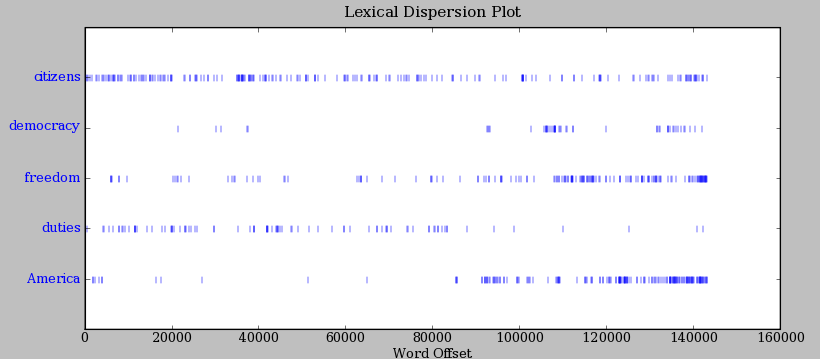
\includegraphics[width=\textwidth]{figs/inaugural}
  \caption{A lexical dispersion plot (of \texttt{citizens},
    \texttt{democracy}, \texttt{freedom}, \texttt{duties}, and
    \texttt{America}) generated using \ac{nltk} from a corpus of
    Inaugural Addresses.  The bottom axis represents the number of
    characters before the word's first appearance.  (From
    \href{http://nltk.org/book/ch01.html}{the documentation}.)}
  \label{fig:disp}
\end{figure}

\clearpage

\printbibliography

\end{document}

%%% Local Variables:
%%% TeX-PDF-mode: t
%%% End:
